\documentclass[fleqn,10pt]{wlscirep}

\usepackage{chemformula}
\usepackage{amsmath}
\usepackage[]{mcode}
\usepackage[utf8]{inputenc}
\usepackage{array}
\usepackage{multirow}
\usepackage{graphicx}
\usepackage{wrapfig}
\usepackage{placeins}
\usepackage{float}
\usepackage{amssymb}
\usepackage{pdfpages}
\usepackage{chemformula}
\usepackage{amsmath}
\usepackage{caption}
\usepackage{subcaption}

\title{Deterministic and Stochastic Dynamics of Hepatic Insulin Receptor Activity}

\author[1]{Timothy Welsh}
\author[2]{Baihan Lin}
\author[1]{Hyeon-Jin Kim}
\author[3]{Trent Nivala}

\affil[1]{Department of Chemistry, University of Washington, Seattle, WA 98195, USA}
\affil[2]{Department of Applied Mathematics, University of Washington, Seattle, WA 98195, USA}
\affil[3]{Department of Biology, University of Washington, Seattle, WA 98195, USA}

\begin{abstract}





\end{abstract}
\begin{document}

\flushbottom
\maketitle
%\thispagestyle{empty}

\section*{Introduction}


\section*{Model}
\begin{figure}[H]
\centering
\includegraphics[width=\textwidth]{figure5frompaper}
\caption{Reproduction of Six-pool model simulation from Figure 5. of original paper}
\label{fig:Reproduction of Figure 5. from original paper} 
\end{figure}


\section*{Results}


\subsection*{Deterministic Dynamics}

\subsection*{Parameter Sensitivity Analysis}

\subsection*{Stochastic Dynamics from Bayesian model}

We are also interested in creating a stochastic model for the insulin receptor system. The first approach is based on the Bayesian  model where the probability of going into next step are based on the amount of transition within a small amount of time. The model is specified as below: \\

In one directional reaction:

\ch{A ->[k_{BA}] B}
\begin{equation}
P(X(t+\Delta t)=B | X=A) = k_{BA}\Delta t
P(X(t+\Delta t)=A | X=A) = 1 - k_{BA}\Delta t
\end{equation}

In two directional reactions:
\ch{C <-[k_{CA}] A ->[k_{BA}] B}
\begin{equation}
P(X(t+\Delta t)=B | X=A) = \frac{k_{BA}}{k_{BA}+k_{CA}}k_{BA}\Delta t
\end{equation}
\begin{equation}
P(X(t+\Delta t)=A | X=A) = 1 - (\frac{k_{BA}}{k_{BA}+k_{CA}}k_{BA}\Delta t + \frac{k_{CA}}{k_{BA}+k_{CA}}k_{CA}\Delta t)
\end{equation}

Implementation details can be found in the supplementary information.

\begin{figure}
    \centering
    \begin{subfigure}[b]{0.3\textwidth}
        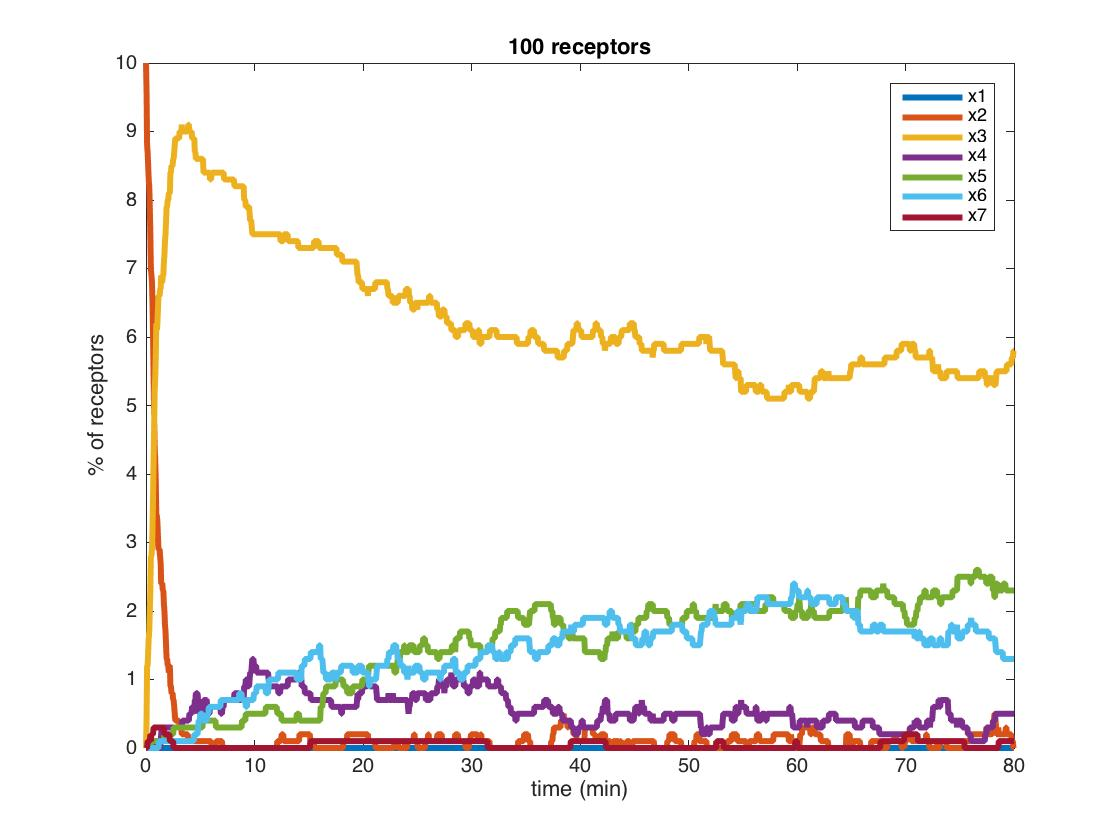
\includegraphics[width=\textwidth]{stoch100}
        \caption{100 receptors}
        \label{fig:stoch100}
    \end{subfigure}
    ~ 
    \begin{subfigure}[b]{0.3\textwidth}
        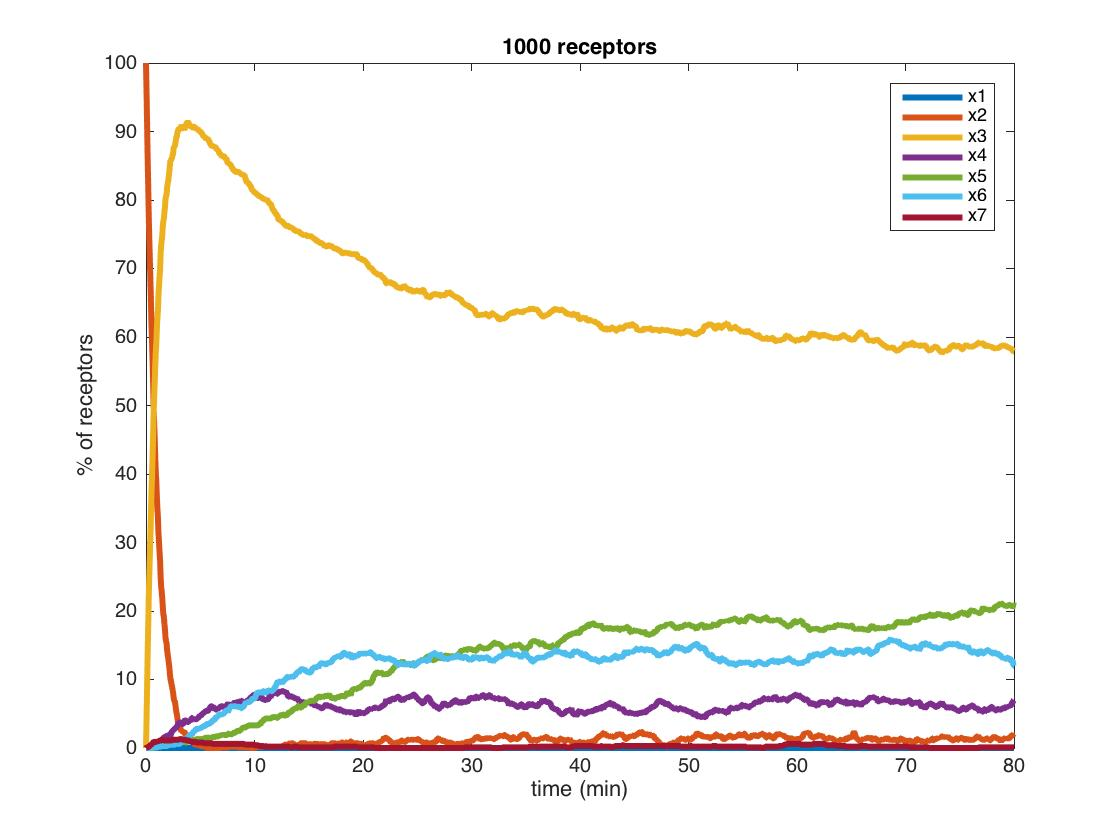
\includegraphics[width=\textwidth]{stoch1000}
        \caption{1000 receptors}
        \label{fig:stoch1000}
    \end{subfigure}
    ~ 
    \begin{subfigure}[b]{0.3\textwidth}
        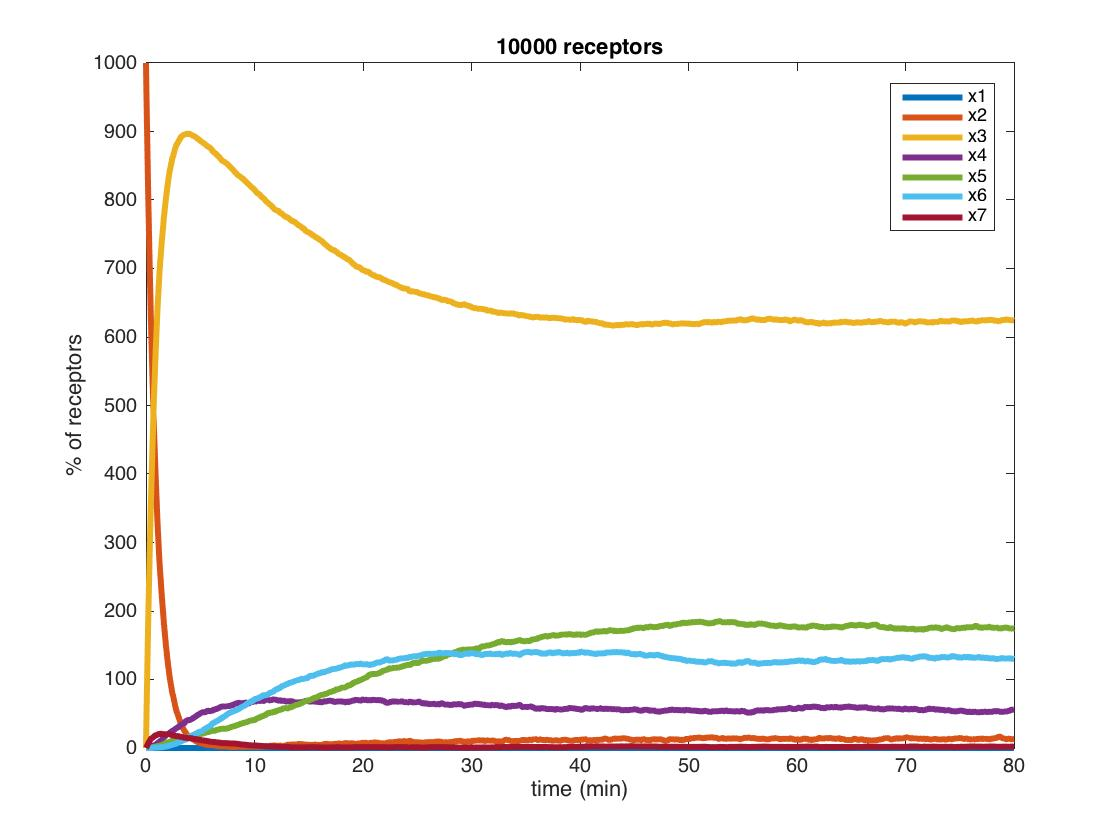
\includegraphics[width=\textwidth]{stoch10000}
        \caption{10000 receptors}
        \label{fig:stoch10000}
    \end{subfigure}
    \caption{Stochastic dynamics from Bayesian model}
    \label{fig:stochsim}
\end{figure}

Based on this stochastic model, in each step, one receptor would make a decision of whether to go to another state or stay in each own state based on the transition probability at that specific time. As shown in Figure \ref{fig:stochsim}, the more receptors to start with, the smoother the simulation curve.

We also explored the dwell time from the function. 

\begin{figure}[ht]
\centering
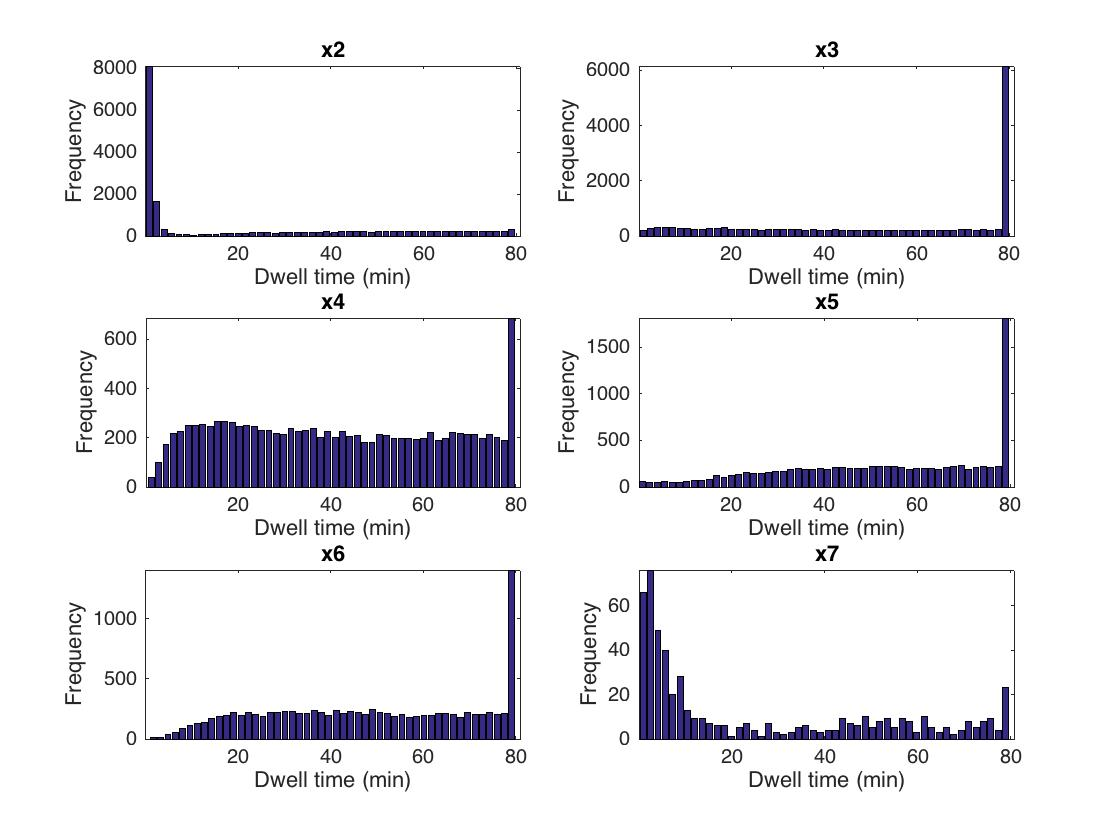
\includegraphics[width=10cm]{dwell10000}
\caption{dwell time from the stochastic simulation of 10000 receptors.}
\label{fig:dwell10000} 
\end{figure}

\subsection*{Stochastic Dynamics from Poissonian waiting time Monte Carlos simulation}

In addition, inspired by Gillespie \cite{GILLESPIE1976403} and Dykeman et al.\cite{Dykeman18052015}, we took a second approach with a logarithmic waiting time assumption towards this system. If we consider all the reactions involved in this system as independent reactions, then under the single-molecule level, within a high resolution of measurement, only one reaction can happen at the same time. Thus, we can assume a Poisson distribution of the waiting time until next reaction

\begin{figure}[ht]
\centering
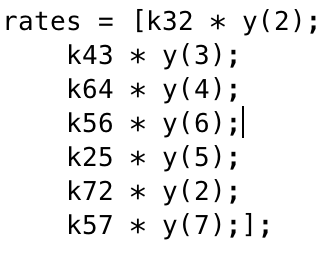
\includegraphics[width=4cm]{rate}
\caption{the reaction rates for each reaction.}
\label{fig:rate} 
\end{figure}

For each reaction type, the mean time till the next reaction occurs again is the inverse of the reaction rate.  Since the rate at which anything will happen is simply the sum of all the reaction rates, which we'll denote by $\lambda$ as shown as Figure \ref{fig:rate}, we also can write the mean time until any reaction occurs as   
   
    \begin{align*}
        \tau_m = \frac{1}{\lambda}    
    \end{align*}
    
Then, under the assumption of a Poisson process, it's fairly straightforward to pick the next most likely reaction and the amount of time until the reaction occurs. For the time, we have
    
    \begin{align*}
        \tau = \frac{1}{\lambda}\log(\frac{1}{U_1})
    \end{align*}
    
for $U_1$ drawn uniformly from the unit interval.  Likewise, if we denote the individual reaction rates as $a_i$ we can select one based on the relative reaction rates by choosing a random variable
    
    \begin{align*}
        r = \lambda*U_2
    \end{align*}
    
which gives for $U_2$ drawn uniformly from the unit interval. This gives us a random variable in the range $(0, \lambda)$  which we can use to select the next reaction $j$ by finding $j$ such that
    
    \begin{align*}
        \sum\limits_0^{j-1} \leq r \leq \sum\limits_0^j
    \end{align*}
    
We then update the current time step with that selected reaction from the transition matrix (Figure \ref{fig:transition}), the number of reactants in all compartments, and go back to the beginning. The update steps are performed by keeping matrices to store the reactant/reaction combinations as well as the number of molecules used in each reaction. Implementation details can be found in the supplementary information.

\begin{figure}[ht]
\centering
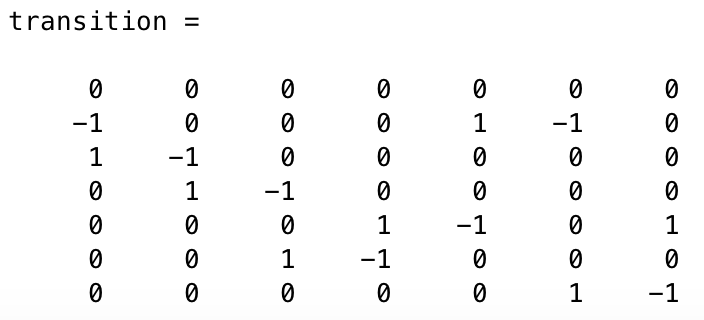
\includegraphics[width=7cm]{transition}
\caption{the transition matrix for this stochastic system.}
\label{fig:transition} 
\end{figure}

For each reaction type, the mean time till the next reaction occurs again is the inverse of the reaction rate.  Since the rate at which anything will happen is simply the sum of all the reaction rates, which we'll denote by $\lambda$, we also can write the mean time until any reaction occurs as   

\begin{figure}
    \centering
    \begin{subfigure}[b]{0.3\textwidth}
        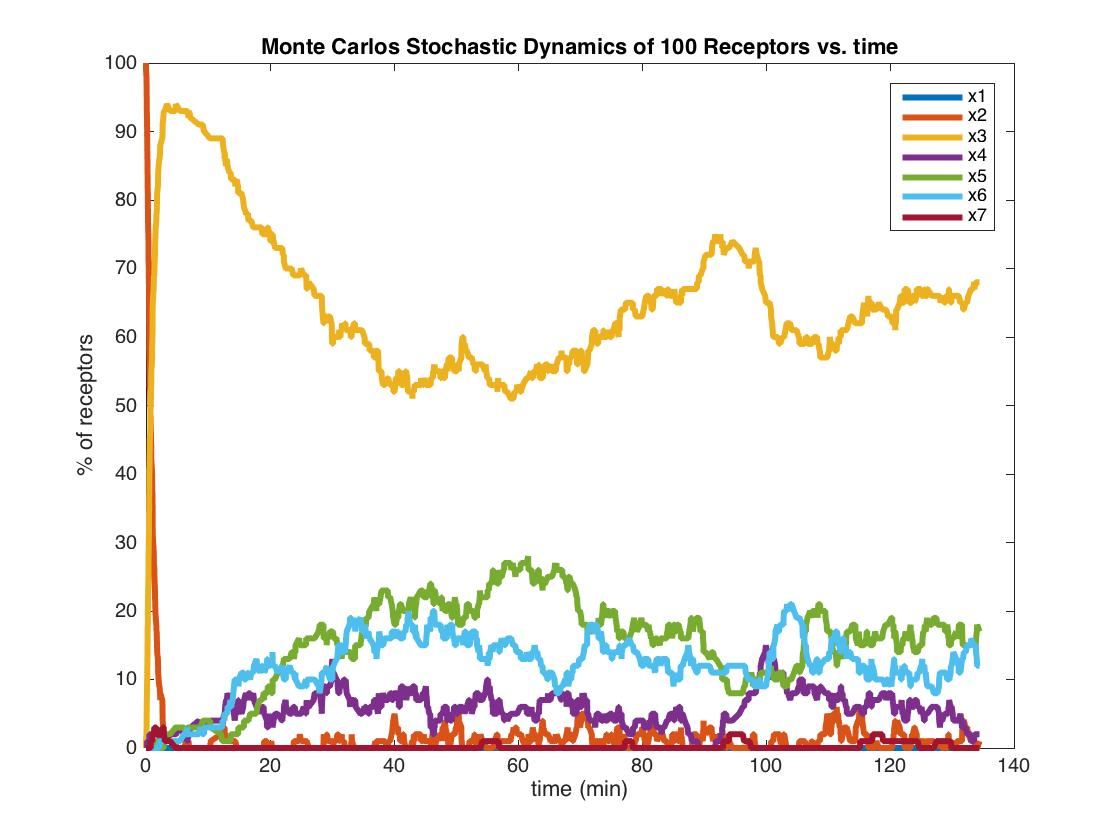
\includegraphics[width=\textwidth]{MC_100_1000}
        \caption{100 receptors 1000 simulation steps}
        \label{fig:MC_100_1000}
    \end{subfigure}
    ~ 
    \begin{subfigure}[b]{0.3\textwidth}
        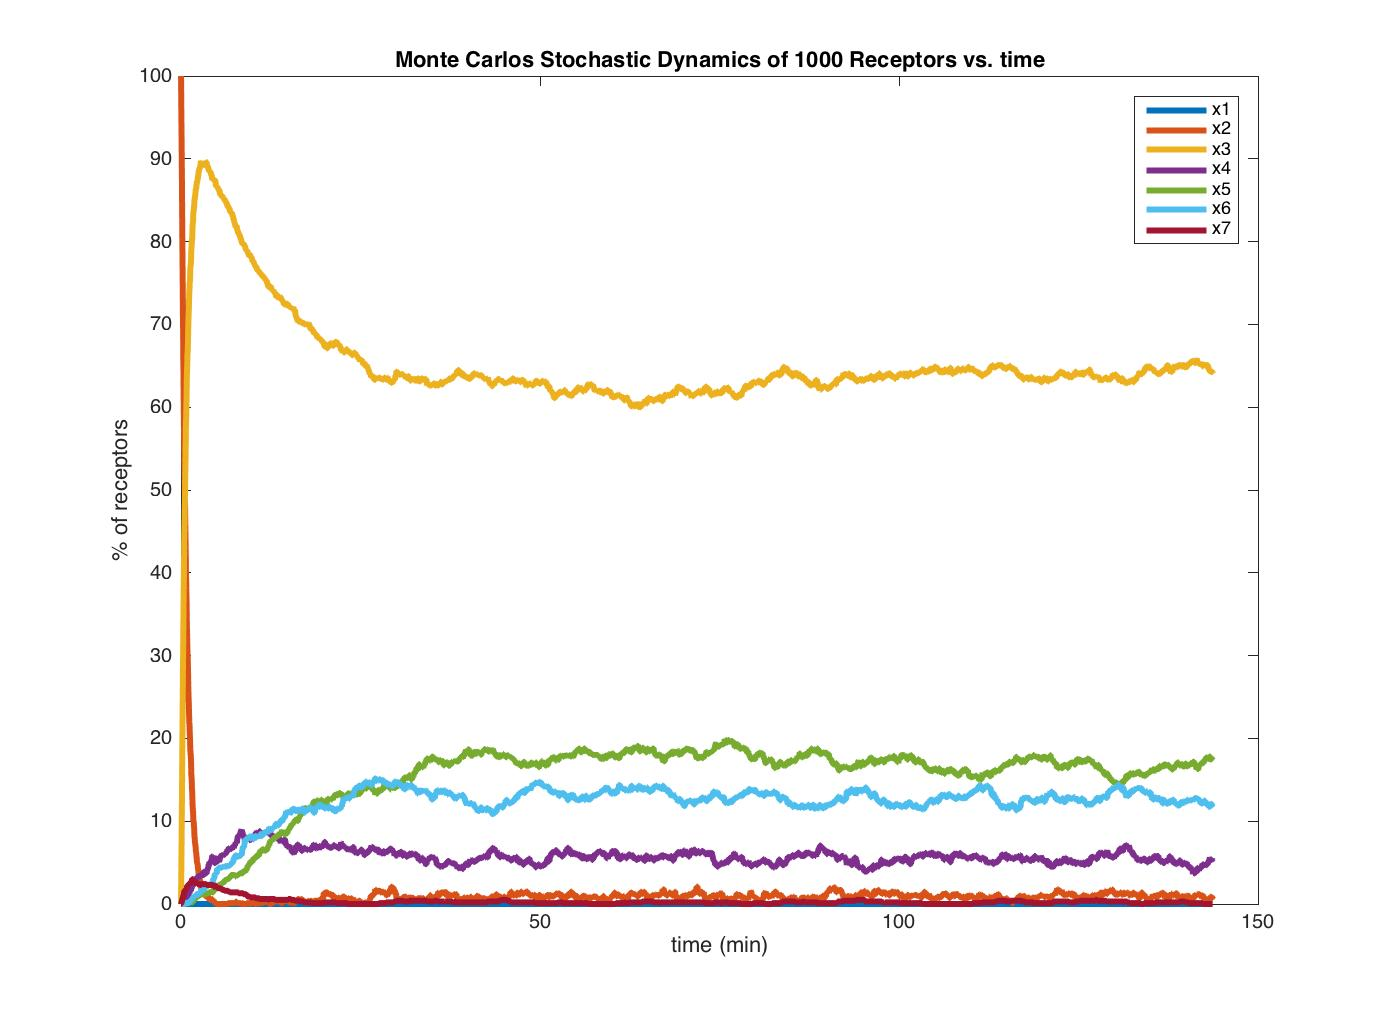
\includegraphics[width=\textwidth]{MC_1000_10000}
        \caption{1000 receptors 10000 simulation steps}
        \label{fig:MC_1000_10000}
    \end{subfigure}
    ~ 
    \begin{subfigure}[b]{0.3\textwidth}
        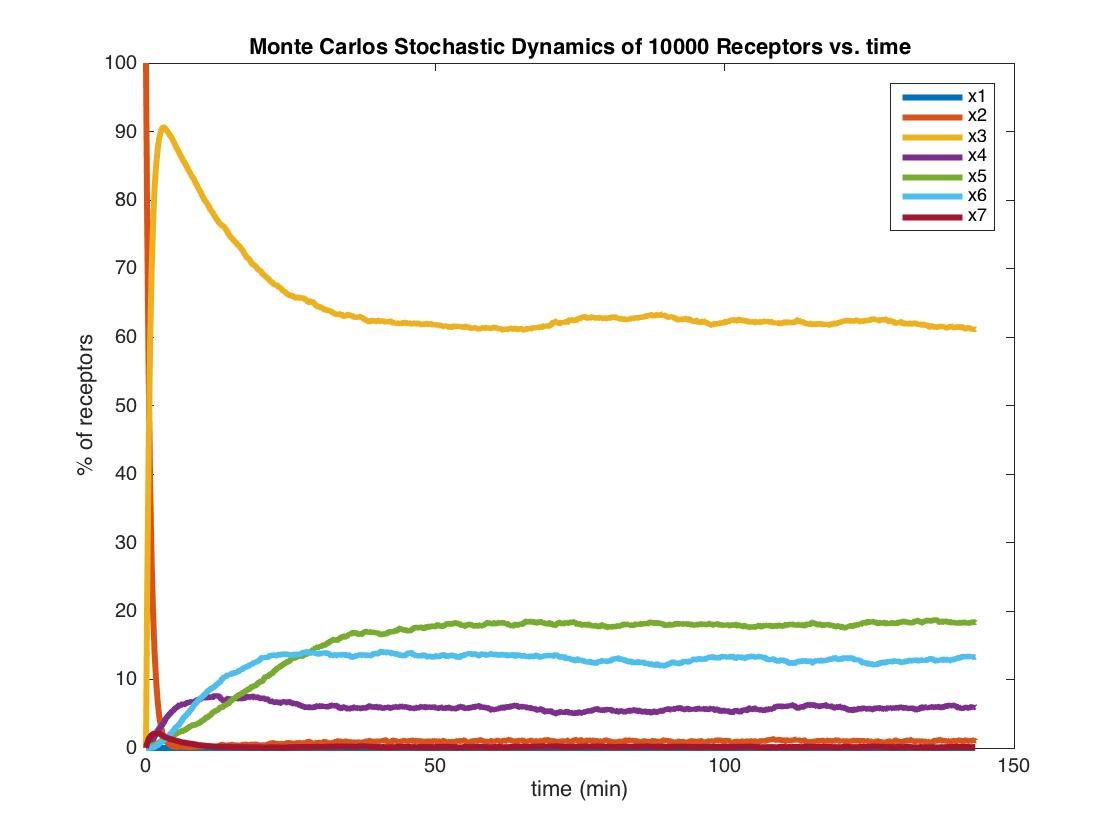
\includegraphics[width=\textwidth]{MC_10000_100000}
        \caption{10000 receptors 100000 simulation steps}
        \label{fig:MC_10000_100000}
    \end{subfigure}
    \caption{the Monte Carlos simulation for the stochastic dynamics of the system}
    \label{fig:MCsim}
\end{figure}

From the stochastic simulation shown in Figure \ref{fig:MCsim}, it seems that the long-term behavior of the insulin receptor activity is relatively stable.

Comparing to the deterministic model, which resembles stochastic simulation dynamics plotted versus steps instead of time, the stochastic model with respect to time shows immediate transition towards equilibrium. To look into further details, since these are rare events, the actual waiting time for a reaction to happen can be pretty short for the first few, but slow down with fluctuation later on.


\section*{Conclusion}

Although the deterministic model works well in capturing the behavior towards equilibrium, the reason why we are also doing stochastic Monte Carlos simulation is that stochastic model is the more accurate model to describe the time-dependent dynamics of the insulin receptor activity. While the deterministic model updates each step in by integrating the system of differential equations, it doesn’t take into account the stochastic nature of biological systems, where the occurrence of each reaction are not continuous, but rather, probabilistic. Statistically speaking, the average behavior resembles the deterministic model, but realistically, stochastic model capture more delicacy regarding time scale.



\bibliography{./sample}

\section*{Acknowledgments}

Thank Prof. Shea-Brown for the great lectures and guidance!

\section*{Appendix}

Supporting MATLAB codes are attached below:


\subsection*{Stochastic Simulation - One Receptor}
\begin{lstlisting}
close all; clear all;

p1=0.0737; %k25
p2=1.29; %k32
p3=0.0411; %k72
p4=0.0212; %k43
p5=0.23; %k64
p6=0.101; %k56
p7=0.23; %k57

delta=0.05; % delta t
Tmax=80;
nums=1000; % number of receptors

p = [p1 p2 p3 p4 p5 p6 p7];
x0 = [0, 1, 0, 0, 0, 0, 0];
tot = zeros(Tmax/delta+1,7);
dwell=zeros(Tmax/delta+1,100);
y=zeros(Tmax/delta+1,7);

for receptors=1:nums
    y = bruteS(x0, p);
    tot = tot + y;
    
    for t=1:(Tmax/delta+1)
        k=find(y(t,:) == 1);
        dwell(t,receptors)=k;
    end
end

%% Simulate the model
figure(1)
set(gca,'FontSize',16)
plot(0:delta:Tmax, tot/10,'LineWidth',3);
title('1000 receptors')
xlabel('time (min)'); 
ylabel('% of receptors');
legend('x1', 'x2', 'x3', 'x4', 'x5', 'x6', 'x7');

%% Dwell times

dwelltimes=zeros(7,1);
list2=[];
list3=[];
list4=[];
list5=[];
list6=[];
list7=[];

for receptors=1:nums
    value=dwell(1,receptors);
    time=1;
    for t=1:(Tmax/delta)
        next = dwell(t+1,receptors);
        if next ~= value || t==(Tmax/delta)
            realdwell = time*delta;
            if value == 2
                list2 = [list2 realdwell];
            elseif value == 3
                list3 = [list3 realdwell];
            elseif value == 4
                list4 = [list4 realdwell];
            elseif value == 5
                list5 = [list5 realdwell];
            elseif value == 6
                list6 = [list6 realdwell];
            else
                list7 = [list7 realdwell];
            time=1;
            end
        else
            time = time + 1;
        end
        value = next;
    end
end

    dwelltimes(2,1:length(list2)) = list2;
    dwelltimes(3,1:length(list3)) = list3;
    dwelltimes(4,1:length(list4)) = list4;
    dwelltimes(5,1:length(list5)) = list5;
    dwelltimes(6,1:length(list6)) = list6;
    dwelltimes(7,1:length(list7)) = list7;

for index=2:7
    xmax=max(dwelltimes(index,:));
    pIndex = dwelltimes(index,:) > 0;
    [nlist,centerlist]=hist(dwelltimes(index,pIndex),50);
    ymax=max(nlist);
    
    figure(2)
    subplot(3,2,index-1)
    bar(centerlist,nlist)
    axis([0.1 xmax+1 0 ymax])
    name=sprintf('x%i', index);
    title(name)
    xlabel('Dwell time (min)')
    ylabel('Frequency')
end
\end{lstlisting}

\subsection*{Stochastic Update - One Receptor}
\begin{lstlisting}
function update = bruteS(y0, p)

Tmax=80;
delta=0.05;
update = zeros(Tmax/delta+1,7);
update(1,:)=y0;

%k25 = p1
%k32 = p2
%k72 = p3
%k43 = p4
%k64 = p5
%k56 = p6
%k57 = p7


x2= p(2) + p(3);
x3= p(4);
x4= p(5);
x5= p(1);
x6= p(6);
x7= p(7);

x=[0 x2 x3 x4 x5 x6 x7];
for t=1:Tmax/delta
    s=rand();
    if update(t,2)==1
        is3 = delta * p(2)*p(2) / x2;
        is7 = delta * p(3)*p(3) / x2;
        if s <= is3
            update(t+1,3)=1;
        elseif s <= is3 + is7
            update(t+1,7)=1;
        else
            update(t+1,2)=1;
        end
    elseif update(t,3)==1
        is4 = delta * x3;
        if s <= is4
            update(t+1,4)=1;
        else
            update(t+1,3)=1;
        end
    elseif update(t,4)==1
        is6 = delta * x4;
        if s <= is6
            update(t+1,6)=1;
        else
            update(t+1,4)=1;
        end
    elseif update(t,6)==1
        is5 = delta * x6;
        if s <= is5
            update(t+1,5)=1;
        else
            update(t+1,6)=1;
        end
    elseif update(t,5)==1
        is2 = delta * x5;
        if s <= is2
            update(t+1,2)=1;
        else
            update(t+1,5)=1;
        end
    else
        is5 = delta * x7;
        if s <= is5
            update(t+1,5)=1;
        else
            update(t+1,7)=1;
        end
    end
end

\end{lstlisting}

\subsection*{Monte Carlos Stochastic Simulation}
\begin{lstlisting}
clear all; close all

p1=0.0737;  %k25
p2=1.29;    %k32
p3=0.0411;  %k72
p4=0.0212;  %k43
p5=0.23;    %k64
p6=0.101;   %k56
p7=0.23;    %k57

Nreceptor = 100000;
p = [p1; p2; p3; p4; p5; p6; p7];
x0 = [0; Nreceptor; 0; 0; 0; 0; 0];

rng(1);

Nstep=10000000;
stptime = zeros(Nstep,1);
time = zeros(Nstep,1);
xall = zeros(Nstep,7);
xall(1,:) = x0;
x = x0;

for step = 1 : Nstep - 1
   [xnew, tau] = MC_stochastic_update(x, p);
   x = xnew;
   stptime(step+1) = tau;
   time(step+1) = time(step) + tau;
   xall(step+1,:) = x;
end

figure(1)
set(gca,'FontSize',16);
plot(time,100*xall(:,1:7)/Nreceptor,'LineWidth',3);
legend('x1','x2','x3','x4','x5','x6','x7');
title('Monte Carlos Stochastic Dynamics of 10000 Receptors vs. time')
xlabel('time (min)'); 
ylabel('% of receptors');
\end{lstlisting}

\subsection*{Monte Carlos Stochastic Ipdate}
\begin{lstlisting}
function [ynew, tau] = MC_stochastic_update(y, p)

k25 = p(1);
k32 = p(2);
k72 = p(3);
k43 = p(4);
k64 = p(5);
k56 = p(6);
k57 = p(7);

rates = [k32 * y(2);
    k43 * y(3);
    k64 * y(4);
    k56 * y(6);
    k25 * y(5);
    k72 * y(2);
    k57 * y(7);];

lambda = sum(abs(rates));

transition = [0 0 0 0 0 0 0;
    -1 0 0 0 1 -1 0;
    1 -1 0 0 0 0 0;
    0 1 -1 0 0 0 0;
    0 0 0 1 -1 0 1;
    0 0 1 -1 0 0 0;
    0 0 0 0 0 1 -1;];

ynew = y;

tau = log(1/rand()) / lambda;

r = rand()*lambda;

current = 0;
selection = 1;

for it = 1:length(rates)
    current = current + rates(it);
    if current > r
        selection = it;
        disp(selection);
        break;
    end
end

ynew = ynew + transition(:,selection);
ynew = ynew.*[ynew >= 0];

end

\end{lstlisting}

\end{document}